\colorlet{mycolor}{green!10!orange!90!}

This section contains the project analysis done using Alloy. The .als file can be found inside the RASD directory \\
\subsection{Introduction}
The alloy model is focused on the main entities and rules of SS:
\begin{itemize}
	\item User-made reports
	\item Main actors
	\item Rules regarding user-made reports
	\item Rules regarding police intervention
	\item Rules regarding data mining rights
\end{itemize}
While, on the other hand, cross-database interactions have not been modeled and the relation between area and violation has not been modeled in its entirety, as the rules about how to assign a violation to an area are missing.\\
Please also note that, even though Authorities actually are users, this part has been omitted in the model for simplicity of description and analysis of the model itself.\\  
\\
\subsection{Signatures}
\textcolor{blue}{sig}
\textcolor{green}{Boolean}\{\} \\
\textcolor{blue}{sig}
\textcolor{green}{True}
\textcolor{blue}{extends}
\textcolor{green}{Boolean}\{\} \\ 
\textcolor{blue}{sig}
\textcolor{green}{False}
\textcolor{blue}{extends}
\textcolor{green}{Boolean}\{\} \\
\textcolor{blue}{sig}
\textcolor{green}{Photo}\{\} \\
\textcolor{blue}{sig}
\textcolor{green}{Person}\{ \\
\} \\
\textcolor{blue}{sig}
\textcolor{green}{Plate}\{\} \\
\textcolor{blue}{sig}
\textcolor{green}{Vehicle}\{ \\
plate: \textcolor{blue}{lone} Plate,\\
ownedby: \textcolor{blue}{one} Person\\
\} \\
\textcolor{blue}{sig}
\textcolor{green}{User}\{ \\
person: \textcolor{blue}{one} Person,\\
areaOfInterest: \textcolor{blue}{one} Area\\ 
\} \\
\textcolor{blue}{sig}
\textcolor{green}{GPScoords}\{ \\
latitude: \textcolor{blue}{one} Int,\\
longitude: \textcolor{blue}{one} Int\\ 
\} \\
\textcolor{blue}{sig}
\textcolor{green}{Intervention}\{\} \\
\textcolor{blue}{sig}
\textcolor{green}{Area}\{ \\
reportsInside: \textcolor{blue}{set} Report,\\
dangerLevel: \textcolor{blue}{one} Int\\ 
interventions: \textcolor{blue}{set} Intervention\\
\} \{\#interventions>0 implies \#reportsInside>0\}\\
\textcolor{blue}{sig}
\textcolor{green}{PositionAndTime}\{ \\
coords: \textcolor{blue}{one} GPScoords,\\
time: \textcolor{blue}{one} Int\\ 
\}\{time>=0 and time<7\} \\
Note: the numbers related to time have been diminished in value for analysis performance reason\\
\textcolor{blue}{abstract sig}
\textcolor{green}{ViolationType}\{\} \\
\textcolor{blue}{sig}
\textcolor{green}{ExpiredTicket}
\textcolor{blue}{extends}
\textcolor{green}{ViolationType}\{\} \\
\textcolor{blue}{sig}
\textcolor{green}{UnauthorizedParking}
\textcolor{blue}{extends}
\textcolor{green}{ViolationType}\{\} \\
Note: UnauthorizedParking and ExpiredTicket are just two examples of the violations that may occurr\\
\textcolor{blue}{sig}
\textcolor{green}{Violation}\{ \\
vehicle: \textcolor{blue}{one} Vehicle,\\ 
positionAndTime: \textcolor{blue}{one} PositionAndTime,\\
violationType: \textcolor{blue}{one} ViolationType,\\
photo: \textcolor{blue}{one} Photo,\\
writtenPlate: \textcolor{blue}{one} Plate\\
\}\ \\
Note: vehicle represents the information retrived from the photo by the system, crossed with the database of car owners; on the other hand writtenPlate is the plate that the user that made the report wrote in it\\
\textcolor{blue}{sig}
\textcolor{green}{Report}\{\\
maker: \textcolor{blue}{one} User,\\
takenCareOf: \textcolor{blue}{one} Boolean,\\
violation: \textcolor{blue}{one} Violation,\\
dispatchedOfficer: \textcolor{blue}{lone} Policeman\\
\}\\
\textcolor{blue}{sig}
\textcolor{green}{Authority}\{\\
person: \textcolor{blue}{one} Person\\
\} \\
\textcolor{blue}{sig}
\textcolor{green}{MunicipalAuthority}\{\\
trackedUsers: \textcolor{blue}{set} User\\
trackedArea: \textcolor{blue}{set} Area\\
trackedVehicles: \textcolor{blue}{set} Vehicle\\
\} \\
\textcolor{blue}{sig}
\textcolor{green}{Policeman}
\textcolor{blue}{extends}
\textcolor{green}{Authority}\{\}\\
\textcolor{blue}{sig}
\textcolor{green}{Ticket}\{ \\
segnalations: \textcolor{blue}{one} Segnalation,\\
policeman: \textcolor{blue}{one} Policeman,\\
issuedTo: \textcolor{blue}{one} Person\\
\}\\
\\
\subsection{Functions}
\textcolor{blue}{fun}
\textcolor{mycolor}{getCoords} [s:Segnalation]:GPScoord\{\\
s.violation.positionAndTime.coords\\
\}\\
\textcolor{blue}{fun}
\textcolor{mycolor}{getTime} [s:Segnalation]:Int\{\\
s.violation.positionAndTime.time\\
\}\\
\\
\subsection{Facts}
\textcolor{blue}{fact}
\textcolor{mycolor}{booleanValue}\{\\
\#True=1 and \#False=1 and \#Boolean=2 and \\
(all b:Boolean | b=True or b=False) and\\
(no b: Boolean | b in True and b in False)\\
\}\\
\textcolor{blue}{fact}
\textcolor{mycolor}{uniqueFoto} \{\\
all p1: Photo | no disj s1, s2 : Violation | s1.photo=p1 and s2.photo=p1\\
\}\\
\textcolor{blue}{fact}
\textcolor{mycolor}{noLonePhoto} \{\\
all p1:Photo | p1 in Violation.photo\\
\}\\
\textcolor{blue}{fact}
\textcolor{blue}{fact}
\textcolor{mycolor}{noSamePlate} \{\\
no disj vei1, vei2: Vehicle | vei1.plate=vei2.plate\\
\}\\
\textcolor{blue}{fact}
\textcolor{mycolor}{noDoubleJob} \{\\
no p:Person | p in MunicipalAuthority.person and p in Policeman.person\\
no disj p1, p2: Policeman| p1.person=p2.person\\
no disj ma1, ma2: MunicipalAuthority | ma1.person= ma2.person\\
no disj u1, u2: User| u1.person=u2.person\\
\}\\
\textcolor{blue}{fact}
\textcolor{mycolor}{cityLimits} \{\\
all gps: GPScoord | gps.latitude>0 and gps.longitude>0 and\\
gps.latitude<7 and gps.longitude<7\\
\}\\
\textcolor{blue}{fact}
\textcolor{mycolor}{noDoubeCoordinates} \{\\
all c1: GPScoord | no c2: GPScoord | c1 != c2 and\\ c1.longitude=c2.longitude and c1.latitude= c2.latitude\\
\}\\
\textcolor{blue}{fact}
\textcolor{mycolor}{areaProperties} \{\\
all a: Area| \#a.reportsInside>=0 and\\ a.dangerLevel=\#a.reportsInside\\
\}\\
\textcolor{blue}{fact}
\textcolor{mycolor}{noMissmatchingPlates} \{\\
all v: Violation| v.vehicle.plate=v.writtenPlate\\
\}\\
\textcolor{blue}{fact}
\textcolor{mycolor}{allPlates} \{\\
\#Violation.writtenPlate=\#Vehicle\\
\}\\
\textcolor{blue}{fact}
\textcolor{mycolor}{violationTypeCardinality} \{\\
\#ViolationType=2 and \#ExpiredTicket=1 and \#UnauthorizedParking=1\\
\}\\
\textcolor{blue}{fact}
\textcolor{mycolor}{noViolationWithSamePhoto} \{\\
all disj v1, v2: Violation| v1.photo=v2.photo\\
\}\\
\textcolor{blue}{fact}
\textcolor{mycolor}{noReportsDuplicate} \{\\
no disj r1, r2: Report| r1.violation=r2.violation\\
\}\\
\textcolor{blue}{fact}
\textcolor{mycolor}{allSegnalationsInAnArea} \{\\
all s: Segnalation | s in Area.segnalationsInside\\
\}\\
\textcolor{blue}{fact}
\textcolor{mycolor}{eitherAllTakenCareOrNone} \{\\
all s1, s2: Report | (getCoords[s1]=getCoords[s2] and\\ getTime[s1]=getTime[s2] and s1.violation.writtenPlate=s2.violation.writtenPlate \\
and s1.violation.violationType=s2.violation.violationType) implies\\ (s1.takenCareOf=s2.takenCareOf and s1.dispatchedOfficer=s2.dispatchedOfficer))\\
\}\\
Note that in reality the constraints on location and time of violation would be different. As a matter of fact, SS would leave a margin for GPS coordinates and time of segnalations, but for analysis complexity reasons those bounds have been simplified in an equality relation.\\
\textcolor{blue}{fact}
\textcolor{mycolor}{sameVehicle} \{\\
all disj s1, s2 : Report | all t: Ticket |\\
(s1 in t.report and s2 in t.report) implies s1.violation.vehicle=s2.violation.vehicle\\
\}\\
\textcolor{blue}{fact}
\textcolor{mycolor}{takenCareOfRule} \{\\
all s: Report |
s in Ticket.segnalations iff s.takenCareOf=True\\
\}\\
\textcolor{blue}{fact}
\textcolor{mycolor}{rightPersonBilled} \{\\
all t: Ticket| t.issuedTo=t.report.violation.vehicle.ownedby\\
\}\\
\textcolor{blue}{fact}
\textcolor{mycolor}{noDoubleBilling} \{\\
all t1: Ticket| all s: Report|
s in t1.report implies no t2:Ticket| t2 != t1 and s in t2.report\\
\}\\
\textcolor{blue}{fact}
\textcolor{mycolor}{dispatchedOfficerWritesTheTicket} \{\\
all t: Ticket| t.policeman=t.report.dispatchedOfficer\\
\}\\
\textcolor{blue}{fact}
\textcolor{mycolor}{ifTakenCareThenOfficerDispatched} \{\\
all r: Report| r.takenCareOf implies \#r.dispatchedOfficer=1\\ 
\}\\
\textcolor{blue}{fact}
\textcolor{mycolor}{noMunicipalDBNoTickets}\{\\
\#Ticket>0 implies all v:Vehicle| v.ownedby=1\\
\}\\
\subsection{Assertions}
\subsubsection{G1}
\textcolor{blue}{assert}
\textcolor{mycolor}{eachSegnalationHasOneAndOnlyPhoto} \{\\
all disj s1, s2: Violation|\\ 
\#s1.photo=1 and \#s2.photo=1 and s1.photo != s2.photo
and \#Photo=\#Report\\
\}\\
\subsubsection{G2}
\textcolor{blue}{assert}
\textcolor{mycolor}{dataMining} \{\\
all u: User| all ma: MunicipalAuthority|\\
\#u.areaOfInterest>=0 and \#ma.trackedAreas>=0 and\\ \#ma.trackedUsers>=0 and \#ma.trackedVehicles>=0\\
\}\\
\subsubsection{G3}
\textcolor{blue}{assert}
\textcolor{mycolor}{everySegnalationHasOneAndOnlyPlate} \{\\
    all disj s1, s2: Violation|\\
s1.writtenPlate=s2.writtenPlate iff s1.vehicle=s2.vehicle\\
\}\\
\subsubsection{G4}
\textcolor{blue}{assert}
\textcolor{mycolor}{everySegnalationHasTimeAndPlace} \{\\
all s1: Violation|\\
\#s1.positionAndTime=1 and \#s1.positionAndTime.coords=1 and \#s1.positionAndTime.time=1 and\\ 
\#s1.positionAndTime.coords.latitude=1 and \#s1.positionAndTime.coords.longitude=1\\
\}\\
\subsubsection{GA1.2}
\textcolor{blue}{assert}
\textcolor{mycolor}{interventionsSuggested} \{\\
all a: Area| \#a.interventions>=0\\
\}\\
\subsubsection{GA2.4}
\textcolor{blue}{assert}
\textcolor{mycolor}{ticketToVehicleOwner} \{\\
all v:Vehicle | all s: Report | all t: Ticket|\\
(s in t.segnalations and v = s.violation.vehicle) implies t.issuedTo=v.ownedby\\
\}\\
\\
\subsection{World}
\textcolor{blue}{pred}
\textcolor{mycolor}{world1} \{\\
\#Vehicle=2\\
\#Report=2\\
\#Ticket=1\\
\#Violation=3\\
\#Policeman=1\\
\#User=1\\
\#MunicipalAuthority=1\\
\#Person=3\\
\#Area=1\\

no p: Person| p in Policeman.person and p in User.person\\
\}\\
\\
\textcolor{blue}{run} world1 for 6\\
\textcolor{blue}{check}
\textcolor{mycolor}{eachSegnalationHasOneAndOnlyPhoto} for 6\\
\textcolor{blue}{check}
\textcolor{mycolor}{dataMining} for 6\\
\textcolor{blue}{check}
\textcolor{mycolor}{everySegnalationHasOneAndOnlyPlate} for 6\\
\textcolor{blue}{check}
\textcolor{mycolor}{everySegnalationHasTimeAndPlace} for 6\\
\textcolor{blue}{check}
\textcolor{mycolor}{intervetionsSuggested} for 6\\
\textcolor{blue}{check}
\textcolor{mycolor}{ticketToVehicleOwner} for 6\\
\newpage
\subsection{Results}
\subsubsection{Checks on assertions}
\begin{figure}[h]
	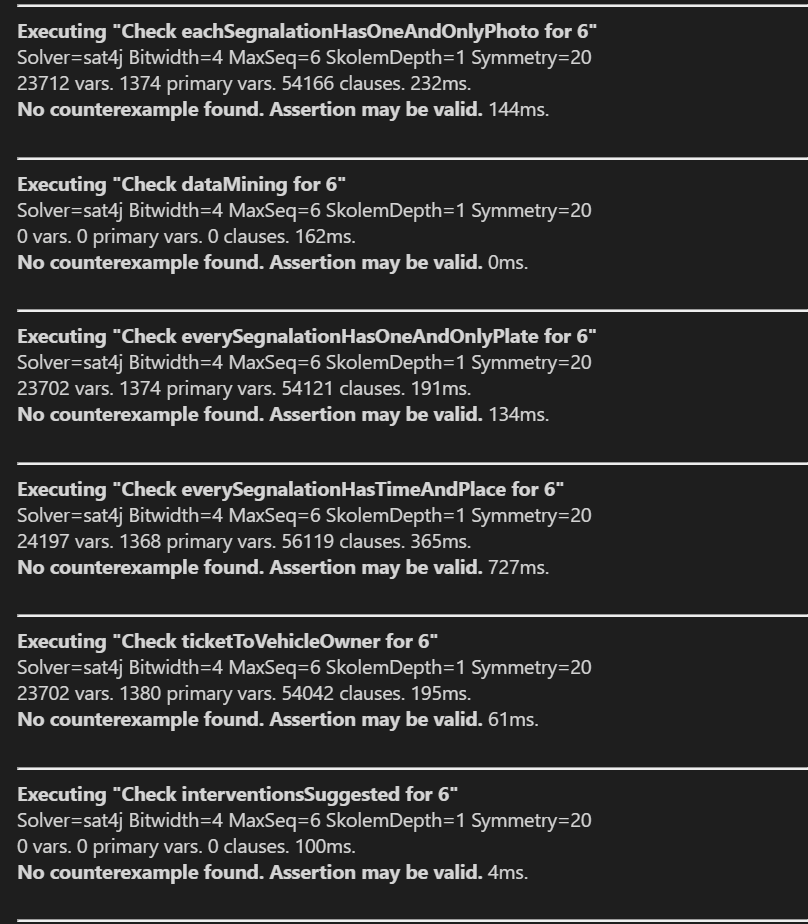
\includegraphics[scale=0.75]{Images/Assert}
\end{figure}
\subsubsection{World generated}
See next page.
\newpage
\begin{figure}[h]
	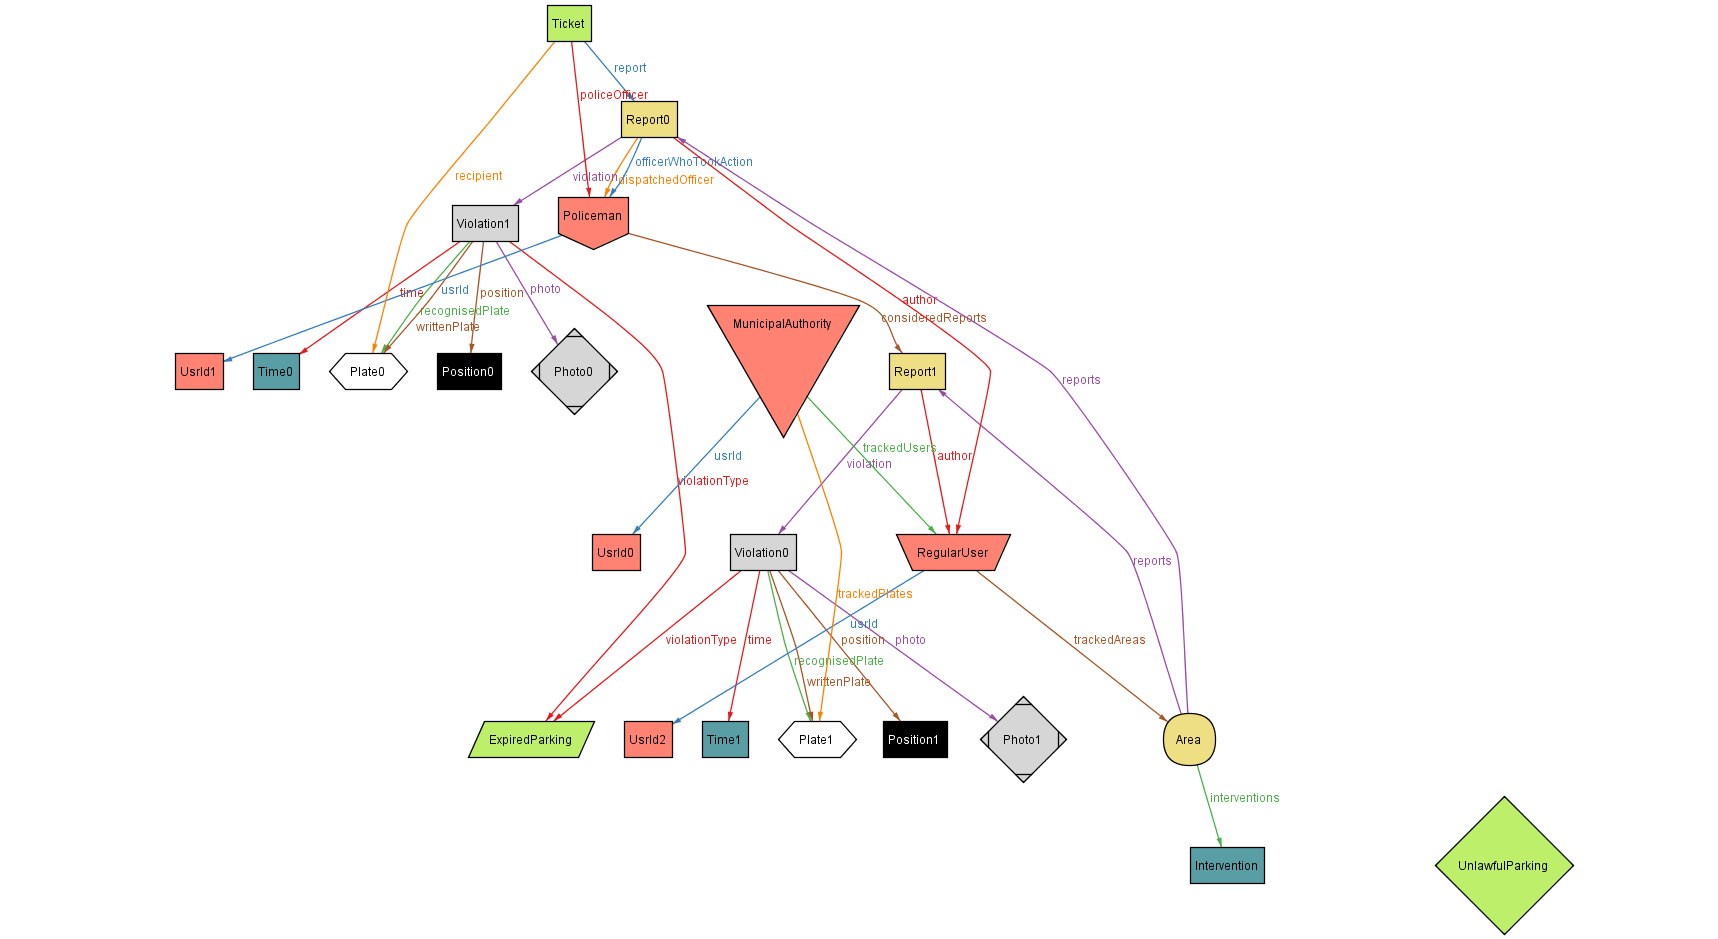
\includegraphics[angle=90, scale=0.45, height=\textheight]{Images/world}
\end{figure}